
\chapter{Software Design}

\section{Einführung}

\subsubsection{Namespace-Übersicht}

\begin{figure}[h!]
    \centering
    \includegraphics[scale=0.27]{Namespace_Uebersicht.png}
    \caption{Die MPD Namespaces im Überblick}
    \label{dd_namespaces}
\end{figure}

\section{,,Das Problem''}

Da die grundlegende Funktionsweise des MPD Server auf einer Client Server Architektur beruht, muss der MPD Client
verschiedene Kommandos wie zum Beispiel \it play, pause, listplaylists \rm etc. an den Server schicken können
und zur gleichen Zeit aber auch auf Änderungen reagieren können, d.h. zum Beispiel wenn sich die Lautstärke ändert,
da jederzeit auch andere Clients oder Server den MPD internen Zustand ändern können.
Diese Änderungen müssen auch anderen Programmteilen bekannt gemacht werden.
Für die Realisierung eignet sich hier das Observer Pattern gut. \footnote{http://de.wikipedia.org/wiki/Observer\_(Entwurfsmuster)}.
\\
Der Client sollte im ,,idle''-Mode möglichst keine Ressourcen verschwenden und auch beim 
trennen und verbinden die entprechenden Änderungen anderen Teilen des Programms mitteilen
können. 
\\

Das MPD Protokoll \footnote{http://www.musicpd.org/doc/protocol/index.html} bietet folgende Möglichkeiten das zu realisieren
\begin{description}
    \item [Periodisch] (zB. alle 500ms) das ,,status'' command absetzen und nach Bedarf auch commands wie ,,currentsong''
        senden
        \\
        \emph{Problem:} Bei langsamen Netzwerkverbindungen erzeugt dies unnötige Netzwerklast 
        Prinzipiell würde sich auf diese Art jedoch die z. B. Musik Bitrate anzeigen lassen, es ist jedoch ein
        wenig komfortabler Weg da hier wieder einmal das Rad neu erfunden werden müsste, denn man müsste manuell rausfinden 
        was genau sich eigentlich geändert hat.
    \item [Nutzung der ,,idle'' und ,,noidle'' commands:]
        ,,idle'' versetzt die Verbindung zum Server in einen Schlafzustand, sobald ,,events'' wie 'player' (also z. B. pause oder play) 
        eintreten, wacht die Verbindung aus diesem Zustand auf und sendet an den Client eine Liste der Events die aufgetreten sind:

\begin{figure}[h!]
    \lstinputlisting[language=bash]{state.txt}
\caption{Eine Beispielantwort des MPD Servers}
\label{dd_state}
\end{figure}

        Einschränkung: Während die Verbindung im idle mode ist kann kein reguläres Kommando wie ,,play'' gesendet werden!
        Sollte man es doch tun wird man vom Server augenblicklich mit einem Disconnect belohnt.
        Die einzige Möglichkeit aus dem idle mode aufzuwachen ist das 'noidle' command das gesendet werden
        kann während die verbindung schlafen gelegt wurde.
        Jedoch gibt es auch hier ein Problem, denn das ,,idle'' command blockiert, sprich es sendet kein ,,OK'' zurück zum Sender.
        Ein Warten auf dieses ,,OK'' würde mit den Wunsch eine bedienbare Oberfläche zu haben kollidieren.
\end{description}

Prinzipiell gibt es 2 Möglichkeiten dieses Problem zu lösen:
\begin{itemize}
    \item Man hält zwei Verbindungen zum Server, eine die Kommandos sendet, eine die stets im ,,idle'' mode liegt,
        Für die Realisierung müssten Threads herangezogen werden. Ein Thread würde dann im Hintergrund auf events lauschen,
        der andere würde zum Abschicken der Kommandos benutzt werden.
        Problem: Es müssen 2 Verbindungen gehandelt werden, was wiederum ein Mehraufwand an Code bedeutet.
        Desweiteren werden Threads benötigt die auch in anderen Bereichen des Programms Lockingmechanismen bedeuten würden.
    \item Man hält eine asynchrone verbindung zu dem server.
        Diese kann das 'idle' command zum server schicken, returned aber sofort. Um nun eine Liste der events zu bekommen setzt man 
        einen ,,Watchdog''auf die asynchrone verbindung an (Vergleiche dazu den Systemaufrug 'man 3 poll'). Da poll() ebenfalls den
        aufrufenden Prozess blockiert, wird Glib::signal\_io() benutzt, das sich in den laufenden MainLoop (*) einhängt und eine 
        Callbackfunktion aufruft sobald auf der verbindung etwas interessantes passiert. Da während des Wartens der MainLoop weiterarbeitet,
        bleibt die GUI (und andere Module) aktiv und benutzbar.
        Problem: Vor dem Senden eines Kommandos wie ,,play'' muss der idle mode verlassen werden.
        Lösung: Man kann das ,,noidle'' Kommando zum verlassen senden, und nach dem Absenden des eigentlichen Kommandos wieder den idle-mode betreten.
\end{itemize}

% Insert telnet session
\lstinputlisting[language=bash]{telnet.txt}

Die Idee zu dieser Implementierung (speziell das Benutzen einer asynchronen Verbindung), kommt von ,,ncmpc'',
der inoffiziellen offiziellen Referenzimplementierung des MPD Mit-Authors \emph{Max Kellermann}.
Vergleiche \href{http://mpd.wikia.com/wiki/Client:Ncmpc}{ncmpc quellcode}: src/gidle.c und src/mpdclient.c

\newpage

\subsection{Verbindungsaufbau}
\begin{figure}[htb!]
	\centering
        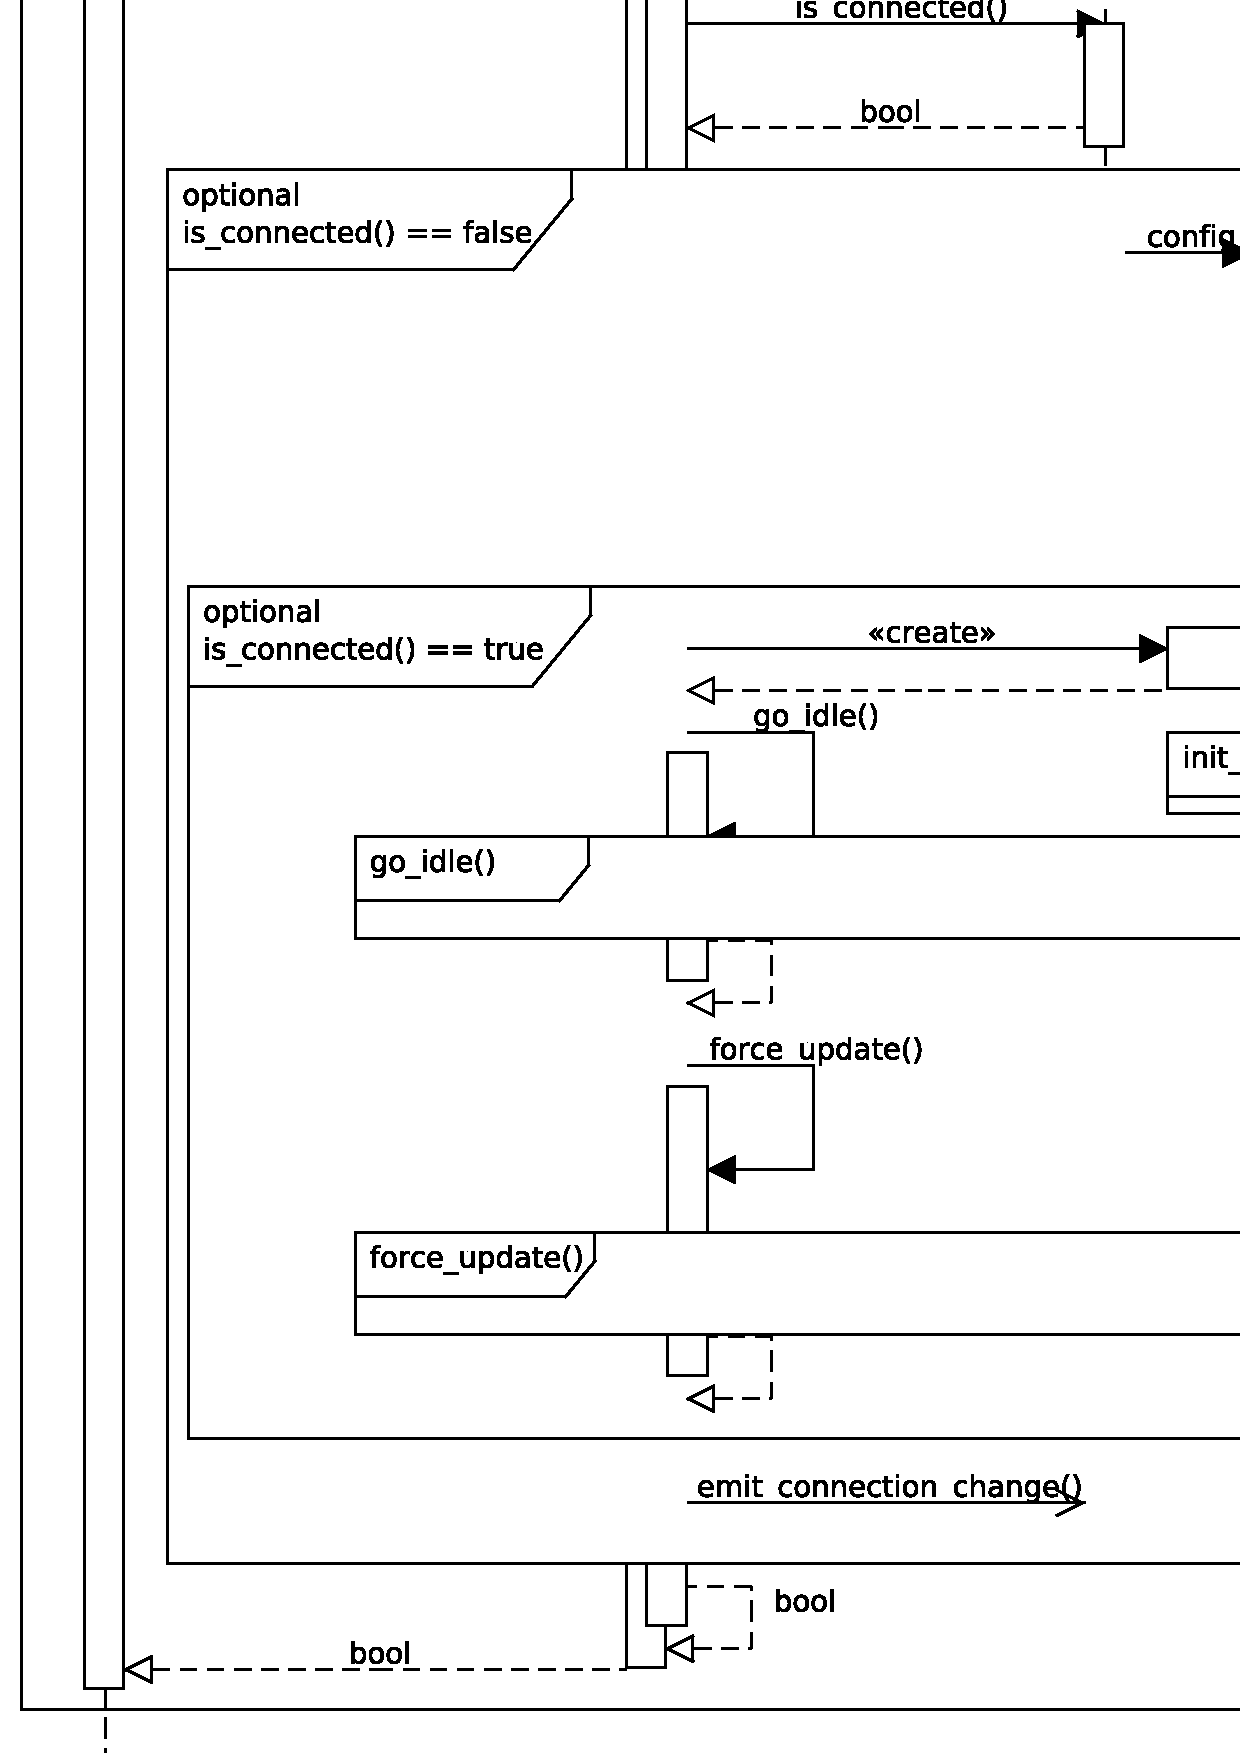
\includegraphics[scale=0.5]{ConnectSequence.pdf}
	\caption{Sequenzdiagramm zum Verbindungsaufbau}
	\label{seq_client_connect}
\end{figure}
Das Sequenzdiagramm stellt den Aufbau der Verbindung beim Start von Freya dar.
\\

\section{Aufbau des Clients}

Aus den oben genannten Anforderungen kann eine grobe Architektur abgeleitet werden.
Zur Realisierung des Observerpatterns wird die sigc++ library benutzt die mit Gtkmm kommt.
Es wird empfohlen die Einführung bis einschließlich Kapitel 2 zu lesen:
\begin{itemize}
\item \url{http://developer.gnome.org/libsigc++-tutorial/stable/ch01.html}
\end{itemize}
Die ersten Einsätze werden auch noch tiefer erklärt.

\newpage
\subsection{Hauptklassen}
\begin{figure}[htb!]
	\centering
        \includegraphics[scale=0.5]{ClientCollab.pdf}
	\caption{Übersichtsklassendiagramm zur Clientstruktur}
	\label{class_client_all}
\end{figure}

\newpage
\subsubsection{Listener}
\begin{figure}[htb!]
	\centering
        \includegraphics[width=\textwidth]{st_ListenerIdleBusy.pdf}
	\caption{Zustandsdiagramm Listener ,,idle/busy''}
	\label{st_listener}
\end{figure}

Der Listener verwaltet alles was mit dem Betreten und Verlassen des ,,Idlemodes'' und den damit verbundenen Events
zu tun hat. Er setzt den eingangs beschriebenen ,,Watchdog'' auf die asynchrone Verbindung an,
und ,,parst'' die entsprechenden Antworten des Servers von Hand (siehe \ref{st_listener}). 
\\
\\
Es folgt eine Liste aller möglichen Events die von libmpdclient definiert werden.
Die Aktionen die passieren müssen, damit diese eintreten, stehen in Klammern.
\begin{itemize}
    \item \small MPD\_IDLE\_DATABASE \it(Datenbank hat sich geändert)\rm
    \item \small MPD\_IDLE\_STORED\_PLAYLIST \it(Änderung an den Playlisten)\rm
    \item \small MPD\_IDLE\_QUEUE \it(Änderung an der Queue: Clear, Add, Remove)\rm
    \item \small MPD\_IDLE\_PLAYER \it(Pause,Stop,Play,Next,Stop,Previous,Seek)\rm
    \item \small MPD\_IDLE\_MIXER \it(Änderung an der Lautstärke)\rm
    \item \small MPD\_IDLE\_OUTPUT \it(An/Ausschalten eines Outputs)\rm
    \item \small MPD\_IDLE\_OPTIONS \it(Random,Repeat,Single,Consume)\rm
    \item \small MPD\_IDLE\_UPDATE \it(Datenbankupdate/rescan wurde gestartet)\rm
\end{itemize}
\normalsize
Bei der Instanzierung des Listeners soll das \textit{sigc::signal} welches das Clientupdate darstellt übergeben werden.
Zudem benötigt der Listener eine Referenz auf MPD::Connection um an die darunter liegende asynchrone Verbindung zu kommen.  
\begin{verbatim}
  Listener(EventNotifier& Notifier, Connection& sync_conn);
\end{verbatim}

Eine weitere Aufgabe des Listeners ist es, das Model MPD::NotifyData aktuell zu halten. Siehe dazu auch MPD::NotifyData.
Bemerkt der Listener Events so ruft er emit() auf dem übergebenen \textit{sigc::signal} auf,
und übergibt als Parameter das aufgetretene Event, sowie eine Instanz von MPD::NotifyData.
\footnote{Als spätere Optimierung könnte das aufgetretene Event übergeben werden um selektiv Daten ,,upzudaten''; Sprich bei einer Lautstärkeänderung muss kein neues Statistikobjekt geholt werden.}
\\
Es folgt eine Liste von Funktionen die der Listener mindestens haben soll.
\\
enter() tritt in den ,,Idlemode'' ein. Es ist ab diesem Punkt nicht mehr erlaubt Kommandos zu senden.
leave() ist das genaue Gegenteil von enter() und verlässt den ,,Idlemode'' sodass Kommandos gesendet werden können.  
is\_idling() sollte selbsterklärend sein.
\begin{verbatim}
       bool enter(void);
       void leave(void);
       bool is_idling(void);
\end{verbatim}

Es soll zudem eine force\_update() Funktion geben die ,,künstlich'' alle Events auslöst.
Dies ist nützlich bei der Initialisierung, bzw. bei ,,Reconnectvorgängen'', wenn die GUI gezwungen werden
soll sich zu updaten.
\begin{verbatim}
       void force_update(void);
\end{verbatim}

\subsubsection{Connection}
\begin{figure}[htb!]
	\centering
        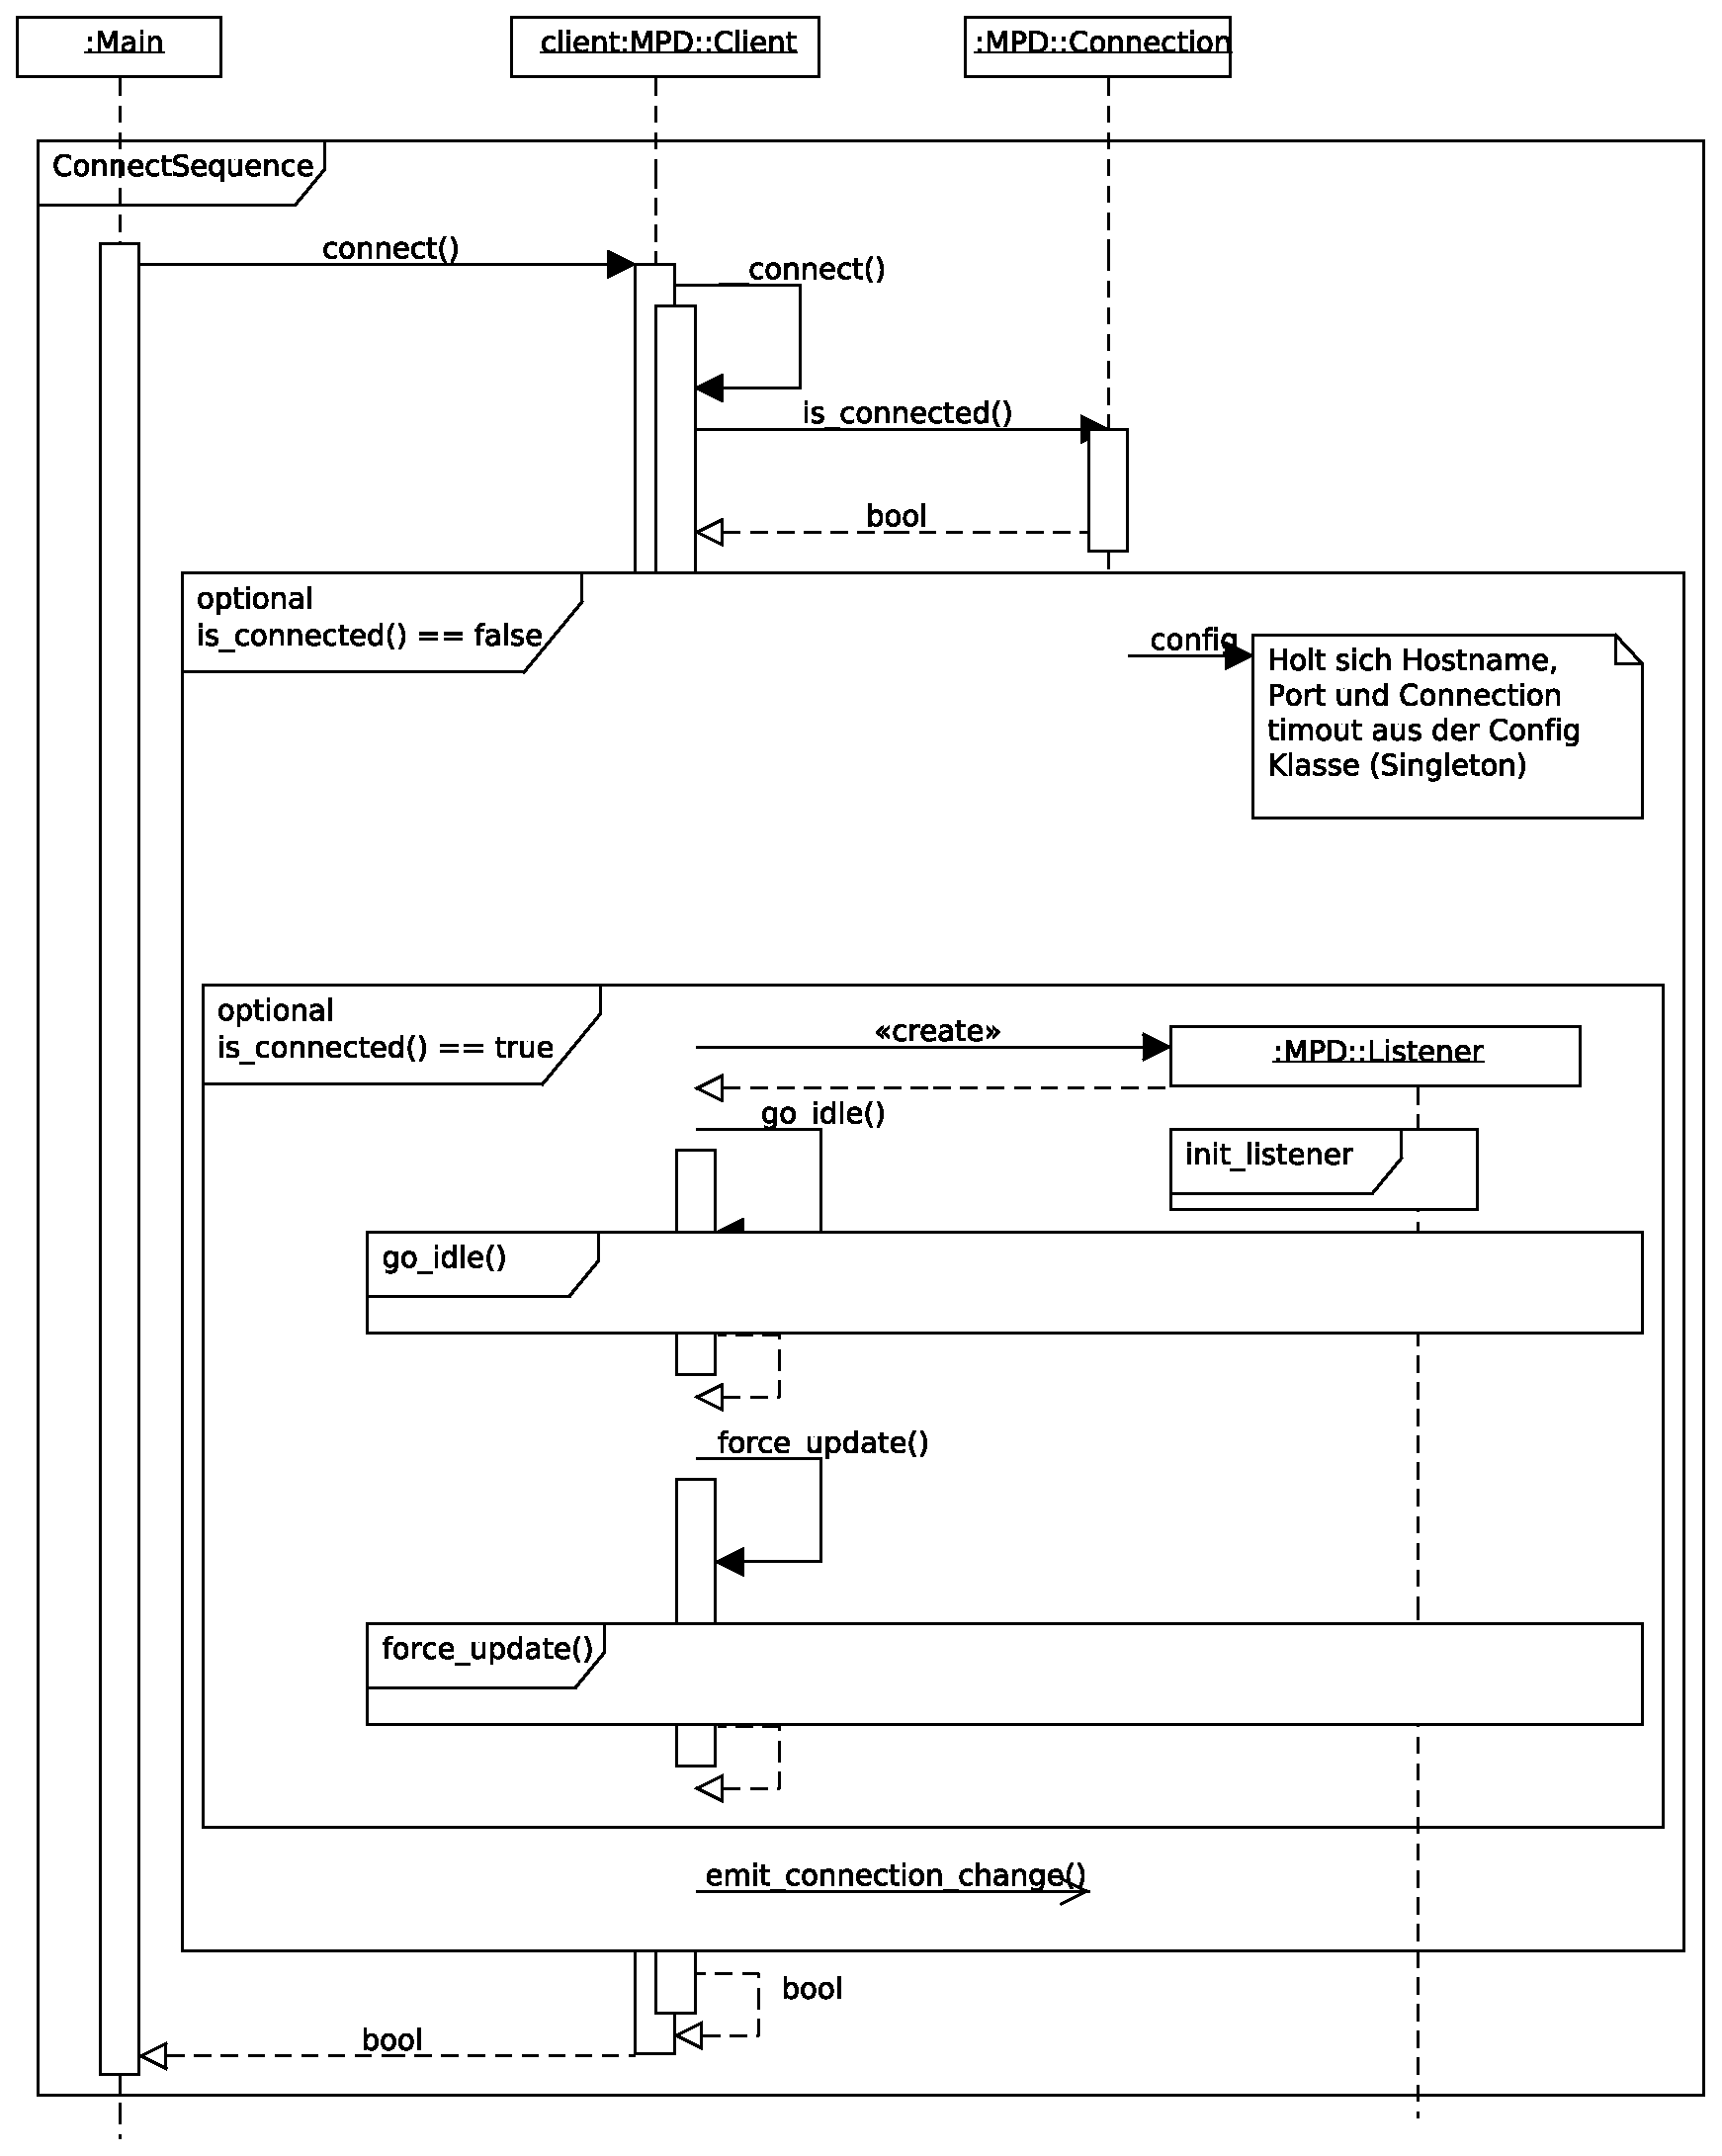
\includegraphics[scale=0.5]{ConnectSequence.eps}
	\caption{Sequenzdiagramm zum Verbindungsaufbau}
	\label{seq_client_connect}
\end{figure}
Diese Klasse stellt eine Art Wrapper um die \textit{mpd\_connection}
\footnote{http://www.musicpd.org/doc/libmpdclient/connection\_8h.html} Struktur von libmpdclient da.
Sie bietet die ,,eigentlichen'' connect() und disconnect() Methoden die letzlich \textit{mpd\_connection\_new()} bzw. \textit{mpd\_connectio\_free()} aufrufen. Siehe \ref{seq_client_connect} für den detaillierten Verbindungsablauf.
Die benötigten Verbindungsdaten (Host, Port, Timeout in Sekunden) holt sich MPD::Connection aus der Config.
\\
Sie hält zudem den letzten Host als Membervariable um feststellen zu können ob sich dieser zwischen 
zwei Verbindungsvorgängen geändert hat. Desweiteren bietet sie eine Schnittstelle um andere Klassen über Fehler in der Verbindung informieren zu lassen (signal\_error()), bzw. um sie zu ,,reparieren'' (clear\_error()).
\\
Es folgt eine Liste von Funktionen die mindestens vorhanden sein sollten.
Ein boolean-Rückgabewert von true zeigt stets Erfolg an.
\\
connect() soll die eigentliche Verbindung herstellen, disconnect() löscht die Verbindung wieder.
get\_connection() liefert einen Pointer auf die darunter liegende C-Struktur.
Alle 3 Funktionen prüfen zudem intern bereits auf Fehler. 
\begin{verbatim}
    bool is_connected(void);
    bool connect(void);
    bool disconnect(void);
\end{verbatim}

Zur Implementierung konkreter Kommandos wird die darunterliegende C-Struktur benötigt.
\textbf{Siehe auch:} AbstractClientExtension
\begin{verbatim}
    mpd_connection * get_connection(void);
\end{verbatim}

Die Connectionklasse soll zudem Schnittstellen bieten um sich für Fehler- und Verbindungsänderungen
zu registrieren. 
Auf den Rückgabewert der folgenden Funktionen kann sigc::signal::connect() aufgerufen werden,
um einen Funktionspointer (bzw. ein ,,Funktor'' um den libsigc++ Begriff zu gebrauchen)
zu registrieren der aufgerufen wird sobald ein Fehler eintritt,
bzw. sich die Verbindung ändert. Die Schnittstellen sollen wie folgt aussehen:
\begin{verbatim}
  typedef sigc::signal<void, bool,mpd_error> ErrorNotify;
  typedef sigc::signal<void,bool,bool> ConnectionNotifier;
    
  ErrorNotify& signal_error(void);
  ConnectionNotifier& signal_connection_change(void)
\end{verbatim}

Die Prototypen entsprechen stets den Templateargumenten in den typedefs:
\begin{verbatim}
  void error_handler(bool is_fatal, mpd_error err_code);
  void conn_change_handler(bool server_changed, bool is_connected); 
\end{verbatim} 

Siehe MPD::BaseClient weiter unten für ein Beispiel wie eine Callbackfunktion registriert wird.
\\
libmpdclient verbietet es weitere Kommandos an den Server zu senden wenn vorher ein Fehler passiert ist.
Fehler müssen zuerst mit \emph{mpd\_connection\_clear\_error()} ,,bereinigt'' werden, 
dies tut check\_error(). Die Funktion wird normal nicht selbst aufgerufen, da sie von allen anderen Funktionen der Klasse
implizit aufgerufen wird. Ist ein Fehler passiert so werden alle Klienten die sich zuvor
mit signal\_error() registriert haben benachrichtigt. 
\begin{verbatim}
  bool check_error(void);
\end{verbatim}

\begin{figure}[htb!]
	\centering
        \includegraphics[scale=0.55]{BaseClientCollab.pdf}
	\caption{Klassendiagramm zu BaseClient}
	\label{collab_base_client}
\end{figure}

\newpage
\subsubsection{BaseClient}

\begin{figure}[htb!]
	\centering
        \includegraphics[width=\textwidth]{st_BaseClientConnection.pdf}
	\caption{Zustandsdiagramm BaseClient Connection}
	\label{st_base_client}
\end{figure}

Diese Klasse bildet die Basis zum eigentlichen Client. Sie kann nicht direkt instanziert werden, da
der Konstruktor protected sein soll.
Sie verwaltet administrative Tätigkeiten wie den eigentlichen Verbindungsaufbau an sich (siehe \ref{seq_client_connect} und \ref{st_base_client}). 
Desweiteren bietet die Klasse einfache Methoden zum Eintreten (go\_idle()) und Verlassen (go\_busy()) des ,,Idlemodes'' an.
Geht die Verbindung verloren, ohne dass \emph{\_\_disconnect()} explizit aufgerufen wurde, so wird versucht sich periodisch zu reconnecten.
Das Intervall in dem diese Versuche geschehen sollen, soll von ,,settings.connection.reconnectinterval'' gelesen werden.
\\
\\
\textbf{Siehe auch:} AbstractClientExtension
\\
MPD::BaseClient soll mindestens folgende public Methoden bieten:
\\
Gibt eine Referenz auf das zugrunde liegende MPD::Connection Objekt zurück. 
Siehe AbstractClientExtension für eine detailliertere Erklärung.
\\
\begin{verbatim}
  Connection& get_connection(void);
\end{verbatim}

Gibt \textit{true} zurück wenn eine Verbindung besteht.
\begin{verbatim}
   bool is_connected(void);
\end{verbatim}

Die get\_status() Funktion soll den letzten aktuellen MPD::Status zurückliefern,
oder \emph{NULL} falls nicht verbunden. Es soll garantiert sein, dass stets ein MPD::Status vorliegt,
wenn is\_connected() wahr ergibt.
\begin{verbatim}        
   Status * get_status(void);
\end{verbatim}

Die folgenden Methoden bieten eine Möglichkeit sich für Clientevents (signal\_client\_update()),
 bzw. für Verbindungsänderungen (signal\_connection\_change()) zu registrieren. 
\begin{verbatim}
  typedef sigc::signal<void,mpd_idle,MPD::NotifyData&> EventNotifier;
  EventNotifier& signal_client_update(void);
        
  typedef sigc::signal<void,bool,bool> ConnectionNotifier;
  ConnectionNotifier& signal_connection_change(void);
\end{verbatim}

Registrieren kann man sich über die sigc::signal::connect() Methode:
\begin{verbatim}
 // Callback Funktion wird bei jedem eingetretenen Event aufgerufen
 void on_client_update(enum mpd_idle event, MPD::NotifyData& data)
 {
    // Tue etwas bei einem 'player' event
    if(event == MPD_IDLE_PLAYER)
    {
        // Gib den Namen des aktuellen Songs aus
        cerr << data.get_song().get_path() << endl;
    }
 }

 // Registrieren der Callbackfunktion
 // - Ableiten von AbstractClientUser macht dies automatisch
 m_Client.signal_client_update().connect(sigc::ptr_fun(on_client_update));
\end{verbatim}

Folgende 3 Funktionen funktionieren genau wie enter(), leave() und force\_update() des Listeners,
allerdings prüfen sie mit Connection::check\_error() vorher stets auf Fehler.
\begin{verbatim}
  void go_idle(void);
  void go_busy(void);
  void force_update(void);
\end{verbatim}

%
%
%
% Zustands oder Sequenzdiagram zum Ausfürehn eines beliebigen Kommandos
% Sprich: go_busy( ) -> send command -> go_idle( )
%
\subsubsection{Client}
Der Client erbt von BaseClient und implementiert konkrete Kommandos wie ,,play'',,,random'' etc.
Er bietet zudem Schnittstellen zur Befüllung der Datenbank, der Queue und des Playlistmanagers indem 
er die abstrakte Klasse \emph{AbstractClientExtension} ausimplementiert.
Er bietet die Methoden connect() und disconnect() die letztendlich von Anwendern der Clientklasse zum Verbinden und Trennen genutzt werden. 
Ist in der config ,,settings.connection.autoconnect'' gesetzt, so connected er sich automatisch.
\\
\\
connect() und disconnect() stellen die öffentliche Schnittstelle zum Verbinden dar.
Sie rufen intern lediglich \_\_connect() bzw. \_\_disconnect() von MPD::BaseClient auf.
\begin{verbatim}
    void connect(void);
    void disconnect(void);
\end{verbatim}

Der Client soll eine Reihe von Kommandos bereitstellen um das Playback zu kontrollieren.
Die ersten 5 der folgenden Funktionen sollten relativ klar sein. 
Zu playback\_pause() sei angemerkt, dass es bei Wiedergabe anhält und bei keiner Wiedergabe wie playback\_play() funktioniert.
playback\_seek() springt in den Song mit der ID song\_id an die Stelle abs\_time in Sekunden.
Die ID des momentan spielenden Songs kann durch get\_status() gefunden werden.
Alle Funktionen, mit Ausnahme von playback\_crossfade), lösen ein ,,player'' Event aus. 
playback\_crossfade löst hingegen ein ,,options'' Event aus.
\begin{verbatim}
    void playback_next(void);
    void playback_prev(void);
    void playback_stop(void);
    void playback_play(void);
    void playback_crossfade(unsigned seconds);    
    void playback_pause(void);
    void playback_seek(unsigned song_id, unsigned abs_time);
    void playback_song_at_id(unsigned song_id);
\end{verbatim}

Die folgenden Funktionen dienen dazu jeweils die \it random, consume, repeat\rm und \textit{single}-Modi umzuschalten.
Alle lösen ein ,,options'' Event aus.
\begin{verbatim}
    void toggle_random(void);
    void toggle_consume(void);
    void toggle_repeat(void);
    void toggle_single(void);
\end{verbatim}

Desweiteren sollten Methoden zum Bearbeiten der Queue vorhanden sein.
\begin{itemize}
    \item \textbf{queue\_add():} Fügt rekursiv den Pfad in der Datenbank hinzu. queue\_add(``/'') entspricht der ganzen Datenbank.
    \item \textbf{queue\_clear():} Leert die gesamte Queue.
    \item \textbf{queue\_delete():} Leert den Song an der Position 'pos'
    \item \textbf{queue\_save\_as\_playlist():} Speichert die aktuelle Queue als Playlist mit dem Namen 'name'
\end{itemize}
\begin{verbatim}
    void queue_add(const char * url);
    void queue_clear(void);
    void queue_delete(unsigned pos);
    void queue_save_as_playlist(const char * name);
\end{verbatim}

database\_update() sendet MPD Server Hinweis um DB zu aktualisieren.
database\_rescan() sendet MPD Server Hinweis um DB neu einzulesen (teuer).
\begin{verbatim}
    void database_update(const char * path);
    void database_rescan(const char * path);
\end{verbatim}

Setzen des ,,volumes'' von 0 bis 100\%.
Die Abfrage des Volumes kann über get\_status() erfolgen.
\begin{verbatim}
    void set_volume(unsigned vol);
\end{verbatim}

Folgende Funktionen sollen von \emph{AbstractItemGenerator} voll implementiert werden.
Siehe daher \emph{AbstractItemGenerator} für eine genaue Erklärung.
\begin{verbatim}
    void fill_queue(AbstractItemlist& data_model);
    void fill_queue_changes(AbstractItemlist& data_model,
                            unsigned last_version,
                            unsigned& first_pos);
    void fill_playlists(AbstractItemlist& data_model);
    void fill_outputs(AbstractItemlist& data_model);
    void fill_filelist(AbstractItemlist& data_model, const char * path);
\end{verbatim}

\subsubsection{NotifyData}
Speichert den aktuellen Status, den aktuellen Song und die aktuelle Datenbankstatistik.
Bietet zudem eine Funktion um entsprechende Daten bei Aufruf zu ,,updaten''.
Die Klasse gehört nach dem MVC Pattern somit der Model-Ebene an.
Der Listener instanziert NotifyData im Konstruktor und gibt an wann sich dieser ,,updaten'' soll (über update\_all()).
\\        

Die folgenden 2 Funktionen garantieren einen validen Rückgabewert, solange eine Verbindung besteht:
\begin{verbatim}
    Status& get_status(void);
    Statistics& get_statistics(void);
\end{verbatim}

\textbf{Anmerkung:} Die folgenden 2 Funktionen sollen NULL zurückgeben können, falls beispielsweise
nichts wiedergegeben wird, oder man im ,,\textit{Singlemode}'' ist.
get\_song() liefert den aktuell spielenden MPD::Song, oder \emph{NULL}.
get\_next\_song() liefert den als nächstes spielenden MPD::Song oder \emph{NULL}.
\begin{verbatim} 
    Song * get_song(void);
    Song * get_next_song(void);
\end{verbatim}

Die update\_all() sollte nur vom Listener aufgerufen werden. Sie aktualisiert den internen Zustand
von NotifyData.
\begin{verbatim}
    void update_all(unsigned event);
\end{verbatim}


\subsection{Weitere Klassen}
Desweiteren gibt es einige weitere Klassen die am Rande eine Rolle spielen,
und meist objektorientierte Wrapperklassen für die C-Strukturen von libmpdclient bereitstellen,
oder im Falle von MPD::AudioOutput und MPD::Playlist eigene Clientkommandos implementieren.

\subsubsection{Song}

Die Song Klasse ist ein Wrapper für mpd\_song Struktur und die dazugehörigen Funktion von libmpdclient. 
MPD::Song soll alle Funktionen von libmpdclient \footnote{http://www.musicpd.org/doc/libmpdclient/song\_8h.html} anbieten.
Diese werden hier nur aufgelistet aber nicht erklärt da sie genau wie ihre Vorbilder funktionieren sollen:

\begin{verbatim}
    const char * get_path(void);
    const char * get_tag(enum mpd_tag_type type, unsigned idx);
    unsigned get_duration(void);
    time_t get_last_modified(void);
    void set_pos(unsigned pos);
    unsigned get_pos(void);
    unsigned get_id(void);
\end{verbatim}

MPD::Song soll zudem eine Funktion bieten um die Metadaten des Songs in einer ,,sprintf'' änhlichen Art als String zurückzuliefern:
\begin{verbatim}
    Glib::ustring song_format(const char* format, bool markup=true);
\end{verbatim}

Ein beispielhafter Aufruf:
\begin{verbatim}
    SomeSong.song_format("Artist is by ${artist}") 
\end{verbatim}

Die Escapestrings die dabei unterstützt werden sollen entsprechen in etwa der \textit{mpd\_tag\_type} Enumeration vom libmpdclient.\footnote{http://www.musicpd.org/doc/libmpdclient/tag\_8h.html\#a3e0e0c332f17c6570ffdf788a685adbf}
Die unterstützten Typen sind somit: \it artist, title, album, track, name, data, album\_artist, genre, composer, performer, comment, disc\rm.
Ist ein Escapestring nicht bekannt, so wird er nicht escaped. Ist der ,,tag'' nicht vorhanden, soll mit ,,unknown'' escaped werden.
\\
Diese Klasse gehört nach dem MVC Paradigma zur Modelschicht.

\subsubsection{Directory}
Die Directory Klasse ist ein Wrapper für mpd\_directory C-Strukutr. Diese wird als Anzeige für ein Verzeichniss benutzt, jedoch nicht als Container für andere Elemente.

Da MPD::Directory die abstrakte Klasse AbstractComposite erweitert muss als
einzige öffentliche Funktion get\_path() implementiert werden:
\begin{verbatim}
    void get_path(void);
\end{verbatim}

Diese Klasse gehört nach dem MVC Paradigma zur Modelschicht.

\newpage
\subsubsection{Statistics}
Die Statistics Klasse ist ein Wrapper für mpd\_stats und
implementiert somit gemäß \url{http://www.musicpd.org/doc/libmpdclient/stats\_8h.html}
folgende Funktionen:
\begin{verbatim}
    unsigned get_number_of_artists(void);
    unsigned get_number_of_albums(void);
    unsigned get_number_of_songs(void);
    unsigned long get_uptime(void);
    unsigned long get_db_update_time(void);
    unsigned long get_play_time(void);
    unsigned long get_db_play_time(void);
\end{verbatim}

Diese Klasse gehört nach dem MVC Paradigma zur Model-Schicht.

\subsubsection{Playlist}
Die Playlist Klasse ist Wrapper für die mpd\_playlist Struktur und
implementiert von \url{http://www.musicpd.org/doc/libmpdclient/playlist\_8h.html} folgende Funktionen:
\begin{verbatim}
    const char * get_path(void);
    time_t get_last_modified(void);
\end{verbatim}

Die Klasse bietet desweiteren  Funktionen zum:
\begin{itemize}
\item Entfernen der Playlist vom Server (Das Playlistobjekt ist danach invalid):
\begin{verbatim}
    void remove(void);
\end{verbatim}

\item Laden der Playlist in die Queue:
\begin{verbatim}
    void load(void);
\end{verbatim}

\item Umbennen der Playlist:
\begin{verbatim}
    void rename(const char * new\_name);
\end{verbatim}

\item Hinzufügen von Songs zur Playlist:
\begin{verbatim}
    void add_song(const char * uri);
    void add_song(MPD::Song& song);
\end{verbatim}
\end{itemize}
Die genannten Funktionen benötigen müssen den idlemode verlassen können,
daher leitet MPD::Playlist von AbstractClientExtension ab.

\subsubsection{AudioOutput}
Die AudioOutput Klasse ist ein Wrapper für mpd\_output, 
implementiert von \url{http://www.musicpd.org/doc/libmpdclient/output\_8h.html} folgende Funktionen:
\begin{verbatim}
    unsigned get_id(void);
    const char * get_name(void);
    bool get_enabled(void);
\end{verbatim}

Die Klasse bietet desweiteren Funktionen zum:
\begin{itemize}
    \item ,,Enablen'' des Ausgabegerätes:
        \begin{verbatim}
            bool enable(void);
        \end{verbatim}
    \item ,,Disablen'' des Ausgabegerätes:
        \begin{verbatim}
            bool disable(void);
        \end{verbatim}
\end{itemize}


enable() und disable() müssen den ,,idlemode'' verlassen können,
daher leitet MPD::AudioOutput von \emph{AbstractClientExtension} ab.
\\
Diese Klasse gehört nach dem MVC Paradigma zur Modelschicht.

\newpage
\subsection{Abstrakte Klassen}
% 
% bei einigen Klassen Klassendiagramme aus Doxygen nehmen
% Einfach damit man sieht wer von diesen Klassen so ableitet
%
\subsubsection{AbstractClientUser}
\begin{itemize}
\item Verwaltet einen Pointer auf die MPD::Client Klasse,
      sodass der Anwender der Klasse dies nicht selbst tun muss.
      Im Konstruktor der Klasse muss eine Referenz auf den Client übergeben werden:
\begin{verbatim}
    AbstractClientUser(MPD::Client& client)
\end{verbatim}      
\item Leitet man von dieser Klasse ab so müssen folgenden Methoden implementiert werden:
\begin{verbatim}
   void on_client_update(enum mpd_idle event, MPD::NotifyData& data);
\end{verbatim}  

     \textit{on\_client\_update()} aufgerufen sobald der Listener eine Änderung feststellt,
     siehe weiter unten ,,Interaktion des Clients mit anderen Modulen''für eine genauere Erklärung.
\begin{verbatim}
   void on_connection_change(bool server_changed, bool is_connected);
\end{verbatim}

     \textit{on\_connection\_change()} wird aufgerufen sobald sich der Client verbunden oder getrennt hat. Im ersten Fall
ist is\_connected true, im anderen false. Sollte sich der Client verbunden haben,
und der neue Server entspricht nicht mehr dem alten so ist auch server\_changed true.
server\_changed soll beim Start des Clients automatisch wahr sein.
\\
Beide Signale werden automatisch durch Konstruktor von AbstractClientUser registriert.
Weiterhin können alle Klassen über den mp\_Client Pointer auf den Client zugreifen.
\end{itemize}

\newpage
\begin{figure}[htb!]
\subsubsection{AbstractItemlist}
    \centering
    \includegraphics[width=\textwidth]{AbstractItemlist.png}
    \caption{Die AbstractItemList}
    \label{c_abstract_item_list}
\end{figure}

Für bestimmte Client Funktionen muss eine Nutzerklasse von \emph{AbstractItemlist} ableiten (siehe \ref{c_abstract_item_list}).
Leitet man ab, so muss die Methode add\_item(AbstractComposite * data) implementiert werden. 
Je nach Bedarf kann über \verb+static_cast<Zieltyp*>(data)+ der entsprechende Datentyp ,,rausgecasted'' werden.
Beim Aufruf von MPD::Client::fill\_queue ruft der Client die add\_item Methode für jeden 
Song den er vom Server bekommt auf. Die ableitende Klasse kann diese dann verarbeiten.

Dadurch werden alle Methoden von AbstractItemGenerator (bzw. die Klassen die davon ableiten) benutzbar.

\subsubsection{AbstractItemGenerator}
%
%
%
% Hier wäre noch ein Sequenzdiagramm nötig,
% zB. für die Funktion fill_outputs( ) - beim Aufruf.

Lässt ableitende Klasse folgende Methoden implementieren:
Jede dieser Methoden ruft MPD::Playlist add\_item() von \emph{AbstractItemlist} auf um ihre Resultate weiterzugeben.
Sie erlaubt den Einsatz des \emph{Proxy-Patterns}.\footnote{http://en.wikipedia.org/wiki/Proxy\_pattern}
Andere Klassen können sich so als Client ,,ausgeben''.
Dies fand Anwendung bei der Klasse ,,DatabaseCache'' weiter unten.
\\
%<Sequenzdiagramm>   
Holt alle Songs der aktuellen Queue.
\begin{verbatim}            
    void fill_queue(AbstractItemlist& data_model);
\end{verbatim}

Holt alle geänderten Songs in der Queue seit der Version last\_version. Die Position des ersten geänderten Songs wird in first\_pos gespeichert. 
\begin{verbatim}
    void fill_queue_changes(AbstractItemlist& data_model,
                            unsigned last_version,
                            unsigned& first_pos);
\end{verbatim}

Holt alle gespeicherten Playlisten vom Server.
\begin{verbatim}              
    void fill_playlists(AbstractItemlist& data_model);
\end{verbatim}

Holt alle Audio Outputs vom Server.
\begin{verbatim}
    void fill_outputs(AbstractItemlist& data_model);
\end{verbatim}

Holt ein Listing aller Songs und Directories aus der Datenbank im Pfad 'path' (nicht rekursiv!)              
\begin{verbatim}
    void fill_filelist(AbstractItemlist& data_model, const char * path);
\end{verbatim}

%<Klassendiagramm, bzw. Klassen die es verwenden von Doxygen nehmen>

%-------------------------------------------
\newpage
\begin{figure}[htb!]
\subsubsection{AbstractComposite}
	\centering
        \includegraphics[width=\textwidth]{AbstractComposite.png}
	\caption{Klassendiagramm zu AbstractComposite}
	\label{c_abstract_composite}
\end{figure}

Vereinheitlicht Zugriff auf Komponenten verschiedenen Typs.
Die abstrakte Klasse (siehe Abb.: \ref{c_abstract_composite}) zwingt seine Kinder dazu eine \emph{get\_path()} Funktion zu implementieren die die Lage im virtuellen Filesystem des Servers angibt.
Der Hauptanwender dieser Klasse ist der Databasebrowser, bzw. der dahinter gelagerte Cache, da AbstractComposite es erlaubt Songs und Verzeichnisse gleich zu behandeln (vgl. Composite Pattern).
\\
Die erbende Klasse muss im Konstruktor angeben, ob es sich bei der Klasse um ein ,,File'' (\emph{true} für MPD::Song) oder um einen ,,Container'' (\emph{false} für MPD::Directory) handelt.
Diese ,,is\_leaf'' Eigenschaft kann später mit der Funktion \emph{is\_leaf()} abgefragt werden.

% <Klassendiagramm für alle Klassen die von AbstractComposite erben, siehe Doxygen>

%-------------------------------------------
\newpage
\begin{figure}[htb!]

\subsubsection{AbstractClientExtension}

	\centering
        \includegraphics[scale=0.8]{AbstractClientExtension.png}
	\caption{Klassendiagramm zu AbstractClientExtension}
	\label{c_abstract_client_extension}
\end{figure}


Diese abstrakte Klasse erlaubt abgeleiteten Klassen ähnlich zum BaseClient eigene Kommandos zu implementieren (siehe \ref{c_abstract_client_extension}).
Dies geschieht indem die abstrakte Klasse eine Referenz auf den BaseClient im Konstruktor erwartet und speichert.
Ableitende Klassen können die \textit{protected} get\_c\_connection() Methode benutzen um eigene Kommandos zu implementieren.

\begin{verbatim}
   AbstractClientExtension(MPD::BaseClient& base_client)
\end{verbatim}

\emph{AbstractClientExtension} wird in diesem Entwurf von MPD::Playlist und MPD::AudioOutput benutzt.
Man kann allerdings darüber diskutieren dass dieses abstrakte Klasse der Modelschicht die Möglichkeit gibt zu ausgefeilte Logik zu implementieren, was nach dem MVC Paradigma nicht sein sollte.  
Da die Logik meist darin besteht einfache Kommandos an den Server zu schicken, wurde dieser Weg gewählt um 
den Entwurf zu vereinfachen.


%=============================================


%% Übergang zu GUI Zeugs..

\section{Interaktion des Clients mit anderen Modulen}
\begin{itemize}
\item Die meisten GUI Klassen leiten von AbstractClientUser ab und speichern daher eine Referenz auf eine Instanz von MPD::Client
        Sie können daher Funktionen wie queue\_add() direkt aufrufen.
\item AbstractClientUser zwingt die abgeleitenden Klassen folgende Funktionen zu implementieren: 
\begin{verbatim} 
   void on_client_update(mpd_idle event, MPD::NotifyData& data)
   void on_connection_change(bool server_changed, bool is_connected)
\end{verbatim}

1) wird aufgerufen sobald der Listener ein Event festgestellt hat. Für jedes eingetretene Event wird 1)
   einmal aufgerufen. 'event' ist dabei eine Enumeration aller möglichen Events, die von libmpdclient 
   vorgegeben werden. \verb+(Siehe auch http://www.musicpd.org/doc/libmpdclient/idle\_8h.html#a3378f7a24c714d7cb1058232330d7a1c)+
   ,,data'' ist eine Referenz auf eine Instanz von MPD::NotifyData. Die benutzenden Klassen können folgenden Funktionen so
   bei Events sofort die aktuellen Änderungen auslesen. 
   \begin{itemize} 
     \item get\_status() gibt den aktuellen MPD::Status
     \item get\_song() gibt den aktuellen MPD::Song
     \item get\_statistics() gibt die aktuellen MPD::Statistics
   \end{itemize} 

2) on\_connection\_change wird vom Client aufgerufen sobald die Verbindung verloren geht.
   Dabei zeigt der übergebene boolean Wert ,,is\_connected'' an ob man connected wurde, oder disconnected wurde.
   ,,server\_changed'' soll dann anzeigen ob der Server derselbe ist beim zuvor geschehenen Connectvorgang.
   Dies ist beim ersten Start stets wahr. ,,server+\_changed'' kann nicht wahr sein wenn ,,is\_connected'' falsch ist.
\item Ableitung von den oben beschriebenen abstrakten Klassen AbstractItemlist und AbstractFilebrowser, um alle Funktionen von AbstractItemGenerator nutzen zu können  
\end{itemize}


\section{Utils und Writer} 

\subsection{Utils}
Im Utils namespace sollen sollen sich folgende Hilfsfunktionen zur Zeit/Datumsumrechnung befinden.

\begin{itemize}
\item Umrechnung in einen Dauer-String Bsp.: ,,4 hours 2 minutes 0 seconds''

\begin{verbatim}
Glib::ustring seconds_to_duration(unsigned long);
\end{verbatim}

\item Umrechnung in einen Timestamp, Bsp: ,,2011-04-02''
\begin{verbatim}
Glib::ustring seconds_to_timestamp(const long);
\end{verbatim}

\item Umwandlung eines Integer Wertes in einen String
\begin{verbatim}
std::string int_to_string(int num); \end{itemize}
\end{verbatim}

\end{itemize}


Diese grundlegenden Funktionen sollen ausgelagert werden damit sie von mehreren Klassen verwendet werden können und um Redundanzen im 
Code zu vermeiden.

\subsection{Writer}

Im Log Namespace befindet sich ebenso die Writer Klasse, welche auch als sog. ,,Utils-Klasse'' Funktionen für alle anderen
Klassen in Namespace bereitstellt. Bei dieser Klasse wurde das Singleton Pattern gewählt, damit diese ohne instanziert werden
zu müssen ,,leicht von überall'' aus erreichbar ist ohne dass vorher eine Instanzierung statt finden muss.
Die Logklasse dient zur Protokollierung von Fehlern und besonderen Ereignissen.  

\begin{figure}[htb!]
Folgende selbsterklärende Makros werden von der Log::Writer Klasse zur Protokollierung bereitgestellt:

\begin{verbatim}
Warning(msg, ...)  _MSG(Log::LOG_WARN, msg, ##__VA_ARGS__)
Info(msg, ...)     _MSG(Log::LOG_INFO, msg, ##__VA_ARGS__)
Fatal(msg, ...)    _MSG(Log::LOG_FATAL_ERROR, msg, ##__VA_ARGS__)
Error(msg, ...)    _MSG(Log::LOG_ERROR, msg, ##__VA_ARGS__)
Debug(msg, ...)    _MSG(Log::LOG_DEBUG, msg, ##__VA_ARGS__)
Success(msg, ...)  _MSG(Log::LOG_OK, msg, ##__VA_ARGS__)
\end{verbatim}
\end{figure}

\section{Config}
%Beschreibung der load/save Funktionalität siehe model_save_load.txt
\subsection{Hauptklassen}

%----------------------------------------------------------------------------------------------

\subsubsection{Path}
Die \emph{Init::Path} Klasse soll für die Initialisierung und das Management der Freya Config Pfade zuständig sein.
Bei der Initialisierung soll überprüft werden ob das Konfigurationsverzeichnis vorhanden ist, wenn nicht wird ein Neues
angelegt und anschließend wird eine default config.xml geschrieben. Eine default config ist im Quellcode als 
globaler konstanter String einkompiliert. (Config::defaultcfg.inl)
\\
\\
Schlägt das Erstellen der Konfigurationsdatei fehl, so soll versucht werden eine entsprechende Fehlermeldung in die Log Datei zu schreiben 
falls diese zuvor erfolgreich angelegt wurde. Zusätzlich sollen DEBUG Ausgaben auf dem Bildschirm angezeigt werden wenn das Programm
über ein Terminal gestartet wird.

\paragraph{Instanzierung der Path Klasse kurz erläutert}
Bei der Instanzierung werden die private Methoden get\_config\_dir() und get\_config\_path() aufgerufen, deren Rückgabewerte werden
als Membervariablen der Init::Path gespeichert. Diese Methoden nutzen die g\_get\_user\_config\_dir() glib Methode
welche den User Pfad nach XDG Standard zurückliefert.
Je nach Funktion, wird an den zurückgegebenen Pfad ein ,,/freya'' für das freya Konfigurationsverzeichnis, ,,config.xml''
für die Konfigurationsdatei oder ,,log.txt'' Logdatei dran gehängt. Bei der Initialisierung wird die dir\_is\_avaiable()
Methode aufgerufen. Diese prüft ob die nötigen Verzeichnisse und Dateien existieren, wenn nicht wird versucht diese
anzulegen. Diese Klasse schreibt DEBUG und ERROR ausgaben auf die Konsole raus, da zum Zeitpunkt der Initialisierung
nicht gewährleistet werden kann dass eine Logdatei angelegt werden konnte.


\paragraph{Die ,,dir is avaiable()'' Methode kurz erläutert}
Diese Methode prüft zuerst über die glib Funktione g\_file\_test() ob ein freya Verzeichnis existiert,
ist dies nicht der Fall werden die privaten Methoden create\_dir() und create\_config() aufgerufen.
Ist ein freya Verzeichnis vorhanden, so wird über die glib g\_file\_test() Funktion geprüft ob die Konfigurationsdatei
config.xml existiert. Existiert diese nicht, so wird die private create\_config Methode() aufgerufen.
Existiert diese, so wird mittels der glib g\_access() Methode geschaut ob und lesbar sowie beschreibar ist, 
wenn dies nicht zugrifft, wird über die glib Funktion g\_warning eine entsprechende Fehlermeldung auf
dem Bildschirm (Konsole) ausgegeben.


\paragraph{Die ,,create config()'' Methode kurz erläutert}
Diese Methode legt einen File Pointer an und erstellt einen file descriptor mit fopen( ,,pfadZurConfig'', ,,w'').
Anschließend wird geprüft ob file pointer ne NULL enthält, ist das der Fall, so ist irgednwas schief gelaufen, eine
entsprechende Warnung wird mittels glib Funktion g\_warning() auf dem Bildschirm ausgegeben.
Ist der File Pointer gültig, wird mit \verb+fwrite(Config::defaultconfig.c_str(),1,Config::defaultconfig.size(),file)+ die
Standard Konfigurationsdatei über den Config::Handler auf die Festplatte in das ensprechende Verzeichnis geschreiben,
der file descriptor mit fclose(file) geschlossen, Speicher freigegeben und eine Erfolgsmessage mit der glib g\_message()
Funktion auf dem Bildschirm ausgegeben.

\paragraph{Die ,,create dir()'' Methode erläutert}
In dieser Methode versucht über die glib Funktion g\_mkdir\_with\_parents(configdir,0755) ein Verzeichnis
mit den rechten 755 (drwxr-r-xr-x) anzulegen. Bei Erfolg wird mit g\_message() eine Erfolgsmeldung auf dem Bildschirm (Konsole)
ausgegeben, andererenfalls eine warnung mit g\_warning().


%----------------------------------------------------------------------------------------------

\subsubsection{Model und Konfigurationsdatei}

Die Freya Konfigurationsdatei soll im simplen XML Format realisiert werden, XML wird gewählt um das Parsen zu vereinfachen und um
ein standardisiertes Format nach außen bereitzustellen. 
\\
Die Konfigurations- und Logdatei soll nach XDG Standard \verb+($XDG_CONFIG_HOME)+ unter \verb+$HOME/.config/freya/<config.xml,log.txt>+ gespeichert werden.
\begin{itemize}
\item \begin{verbatim}
	http://standards.freedesktop.org/basedir-spec/basedir-spec-latest.html#variables
\end{verbatim}
\end{itemize}

Die Optionen in der Konfigurationsdatei sind baumartig nach ,,Domainprinzip'' aufgebaut. Die Konfigurationsdatei unter \ref{c_config}
zeigt exemplarisch einen möglichen Aufbau.


	\lstinputlisting[language=XML]{config.xml}



Die \emph{Config::Model} Klasse gehört nach dem MVC Paradigma zur Model Schicht. Diese Klasse soll die nötigen Daten (Konfigurationsdatei)
die zum Betrieb von Freya nötig sind im Speicher vorhalten und Methoden zum Lesen und Speichern der Konfigurationsdatei auf die Festplatte 
bereit stellen.

Zum Parsen der XML Datei soll hier die C Programmbibliothek libxml2 verwendet werden. Diese Library wurde gewählt, weil sie alle benötigten Funktionen enthält, nach dem ANSI-C Standard implementiert ist
und bereits seit über einem Jahrzehnt Quasi-Standard im C Umfeld ist.

Zu verwendende Libraries:
\begin{itemize}
    \item \url{http://xmlsoft.org/}
    \item \url{http://en.wikipedia.org/wiki/Libxml2}
\end{itemize}

%Hier das Sequenzdiagramm vom Model



\begin{figure}[htb!]
	\centering
  	\includegraphics[scale=0.6]{init.pdf}
	\caption{Initialisierung des Models}
	\label{c_modelinit}
\end{figure}


\subsection{Initialisierung des Models}

 
Über die Init::Path Klasse holt sich das Model bei seiner Instanziierung über die path\_to\_config() Methode
den Pfad zur Konfigurationsdatei, parst diese sowie die default Config und 
initialisiert zwei XML Document Pointer die auf ein DOM Objekt, welches einen Dokumentenbaum enthält, zeigen.
Hierzu werden die load(pathtofile) und die loadDefaulDoc() Methoden der Config::Model Klasse verwendet.
\\   

Anschließend kann man über diese DOM Objekte traversieren und Werte der Konfigurationsdatei lesen oder setzten.
Die default config wurde implementiert um fehlerhaften Werten oder einer kaputten Konfiguration vorzubeugen. Ist ein benötigter Wert
nicht in der User config vorhanden oder ist diese beschädigt so wird auf die default config zugegriffen.
Bei Beendigung des Models wird das aktuelle Objekt als XML Konfigurationsdatei auf die Festplatte geschrieben.
Wie andere Objekte auch, nutzt das Model die Log-Klasse um zu Informationen und Fehler zu protokollieren.


\subsection{Prinzipieller Ablauf der load() Methode}

Beim Instanzieren ruft das Model seine load() Methode auf mit dem aktuellem Pfad auf
in dieser wird als Erstes die libxml2 Methode xmlParseFile(pathtofile) aufgerufen. Diese bekommt den
Pfad zur Konfigurationsdatei übergeben und versucht über den übergebenen Pfad zu das File zu laden.
An den ,,xmlNodePtr curNode'' Pointer wird der Rückgabewert der xmlParseFile() Methode zurückgegeben,
wenn die Operation erfolgareich war, ansonsten \emph{NULL}.

Anschließend wird das geladene Dokument geprüft, ist dieses \emph{NULL} so wird eine entsprechende Fehlermeldung
über den Logwriter in die Logdatei geschreiben, wurde ein gültiger xmlDocPtr zurückgegeben so geschieht folgendes:

\begin{itemize}

\item Der curNode Pointer wird auf das root Element über xmlDocGetRootElement(fileDOc) gesetzt
\item Überprüfung ob das curNode Null ist, trifft das zu, so wird ein Error in die Logdatei über den Log::Writer geschrieben
      allokierter Speicher vom fileDoc mittels xmlFreeDoc(fileDoc) freigegeben und fileDoc auf NULL gesetzet
\item Ist das curNode gültig, so wird mittels der libxml2 Methode xmlStrcmp(curNodeName, ,,freya'') geprüft ob es dem
      root Element ,,freya'' entspricht. Ist dies der Fall wird eine Erfolgsmeldung in die Logdatei geschreiben,
      ansonsten wird eine Fehlermeldung über den Logwriter raus-geschrieben, allokierter Speicher vom fileDoc über xmlFreeDoc(fileDoc)
      freigegeben und die beiden Pointer fileDoc und curNode werden auf \emph{NULL} gesetzt. 
\end{itemize}
%sequenzdiagramm

\subsection{loadDefaultDoc() Methode}
Diese Methode holt sich die default Konfigurationsdatei aus einem einkompilierten String.
Dieser String wird anschließend mittels der libxml xmlParseMemory() geparst und ein xmlDocPtr wird zurückgegeben der als defaultDoc
Membervariable gespeichert wird.

\subsection{Ablauf der save() Methoden zum Speichern des aktuellen xmlDocPtr auf die Festplatte}
Die save() Methode ist eine Wrapper Methode für save(char*, xmlDocPtr). Sie ruft lediglich diese mit dem aktuellen xmlDocPtr
und dem Pfad zur config.xml auf.

Quellen zur Implementierung:
\begin{itemize}
    \item \url{http://xmlsoft.org/tutorial/index.html}
    \item \url{http://student.santarosa.edu/~dturover/?node=libxml2}
\end{itemize}

%
%-------------------------------
%


\subsubsection{Controller}
%Bescheibung der get/set Funktionalität siehe handler_set_get_values.txt
Die Config::Handler Klasse gehört nach dem MVC Paradigma zur Controller Schicht. Diese Klasse soll für das Management bzw für den
Zugriff auf das Model und somit die Konfigurationsdatei zuständig sein. Sie enthält Methoden zum Lesen und Setzen der einzelnen Optionen.
Der Config::Handler wird als Singleton implementiert um einen zentralen Zugriff über eine einzelne Schnittstelle zu ermöglichen.

Der Handler soll einen Pointer als Membervariable auf das aktuelle Model Objekt bekommen um direkten Zugriff auf die Dokument Pointer
zu haben. Desweiteren sollen Wrapper um die get und set value Methoden geschrieben werden um verschiedene Datentypen lesen und setzen zu können, so kann gleich eine ,,Teilvalidierung'' erfolgen.

Der Config::Handler stellt folgende Makros bereit:
    \begin{verbatim}
    CONFIG_SET(x,y) 
    CONFIG_GET(x)   
    CONFIG_SET_AS_INT(x,y) 
    CONFIG_GET_AS_INT(x)   
    CONFIG_SAVE_NOW() 
    CONFIG_GET_DEFAULT(x)
    CONFIG_GET_DEFAULT_AS_INT(x)
    \end{verbatim}

Über die \emph{save\_now()} Methode soll die aktuelle Konfiguration direkt über das Model gespeichert werden können.
Alle Methoden nutzen nach Möglichkeit die Log-Klasse um Informationen und Fehler in der Logdatei zu protokollieren.


\begin{figure}[htb!]
	\centering
  	\includegraphics[scale=0.5]{configset.pdf}
	\caption{Config get vlaue() Ablauf}
	\label{c_configget}
\end{figure}



Grober Ablauf beim setzen einer Integer Wertes:



\begin{itemize}

    \item Aufruf des \verb+CONFIG_SET_AS_INT("settings.connection.port",6667)+ Makros, Url ist ein ustring, Port ein Integer
    \item Über das Makro wird die Wrapper Methode \verb+set_value_as_int(Glib::ustring url,int value)+ aufgerufen
    \item Diese Methode wandelt den Integer Wert in einen String (char*) um und ruft die eigentliche set Methode 
          set\_value(url, wert) auf
    \item Die set\_value(url, wert) Methode holt sich über cfgmodel.getDocPtr(); einen aktuellen Dokument Pointer über die Model
    \item Ist der Dokument Pointer NULL, so kann kein Wert geschrieben werden, also wird über den Log:Writer
          eine entsprechende Warnung in die Logdatei geschreiben.
    \item Bei einem gültigem Dokument Pointer wird  xmlNodePtr cur = xmlDocGetRootElement(doc) aufgeruden,
          diese liefert einen xmlNodePtr (xml node pointer) auf das root Element zurück.
    \item Mittels cur->xmlChildrenNode wird der Pointer auf den folgenden Kinderknoden gesetzt und die traverse() Methode aufgerufen
     \item Nun werden diverse Vorbereitungen getätigt und anschließend rekursiv im Baum nach der übergebenen Url gesucht. Hier wird rekursiv
     der jeweilige Teilstring (teilstring1.teilstring2.teilstring2) gemäß dem Url Aufbau untersucht
           
     \item Wird die Url nicht gefunden oder sind andere Fehler aufgetreten wird ein \emph{NULL Pointer} zurückgegeben
                  und eine entsprechende Fehlermeldung in die Logdatei geschrieben
     \item Wird die die entsprechende Url gefunden, so wird der Optionswert über die Aufruferkette an die set\_value() Methode \emph{returned}.
     Hier wird dann der Wert an die entsprechende Stelle gesetzt.  
\end{itemize}


\begin{figure}[htb!]
	\centering
\includegraphics[scale=0.5]{configget.pdf}
\caption{Config get\_value() Ablauf}
\label{c_configget}
\end{figure}

%-------------------------------------------


Grober Ablauf beim Lesen eines Wertes:
\begin{itemize}


   \item Das Makro \verb+CONFIG_GET("settings.connection.host")+ wird analog dem setzen aufgerufen, dieses ruft die entsprechende Wrapper
   Methode \verb+get_value(Glib::ustring)+ welche die eigentliche \verb+_get_value(Glib::ustring url,bool getdefault)+ Methode aufruft.
   Der zweite Parameter dient dazu der \verb+_get_value()+ Methode mitzuteilen ob der entsprechende Default Wert aus der einkompilierten 
   Konfigurationsdatei oder der Custom User Wert gelanden werden soll.
   \item Die \verb+_get_value()+ Methode entsprechend dem flag, den ,,richtigen'' Dokument Pointer über das Model (analog Setzen eines Integer Wertes)
   \item Bei einen gültigen Pointer wird analog zum Setzen der Dokument Pointer auf das erste Element gesetzt und traverse
      aufgerufen (siehe Setzen eines Wertes).
   \item Kann kein Node ermittelt werden (d.h. cur Pointer zeigte auf NULL nach dem traversieren), so wird eine entsprechende Warnung über den
         Logwriter in die Logdatei geschreiben und anschließend wird die \verb+_get_value(url,true)+ Methode rekursiv mit einem true Flag aufgerufen.
         Aufgrund des true flags wird nun der Dokument Pointer mit den Default Werten über das Model geladen.
    \item Analog zum bisherigen Verlauf beim ,,Lesen eines Wertes'' erfolgt die Suche des Default Wertes. Kann am Ende kein
    Default Wert ermittelt werden so wird an den Aufrufer eine leerer ustring "" zurückgegeben.
\end{itemize}











\section{GUI Elementklassen}

\subsection{Hauptklassen}
Der GManager Namespace enthält Klassen die der Verwaltung und Kontrolle des Hauptfensters von Freya dienen,
jedoch nicht für den eigentlichen Inhalt des Hauptfensters (dies wird vom Browser namespace getan)
Alle Klassen gehören nach dem MVC Paradigma der Controllerschicht an.


\subsubsection{BrowserList}
Zeigt eine Liste von Browsern in der Sidebar.
\begin{itemize} 
\item Bietet eine add() Methode die eine Referenz auf AbstractBrowser erwartet und fügt in der Sidebar hinzu.
\item set() setzt den Browser temporär, ohne ihn hinzuzufügen.
\end{itemize}
Benutzt alle Methoden von AbstractBrowser um dise entsprechen anzuzeigen:
\\
Der Container der im Hauptbereich beim wechseln angezeigt wird
\begin{verbatim}
  Gtk::Widget * get_container();
\end{verbatim}
Welcher Name soll in der Sidebar angezeigt werden?
\begin{verbatim}
  Glib::ustring get_name();
\end{verbatim}
Welche Gtk::Stock::ID soll in der Liste angezeigt werden?
\begin{verbatim}
  Gtk::Stock::ID get_icon_stock_id();
\end{verbatim} 
Ist sichtbar in der Leiste?
\begin{verbatim}
  bool is_visible(); 
\end{verbatim}
Benötigt dieser Browser eine Verbindung zum funktionieren?
\begin{verbatim}
  bool needs_connection(); 
\end{verbatim}

Als View wird ein Gtk::TreeView benutzt, die Browserreferenzen werden in einem Gtk::ListStore gespeichert,
was damit das Model darstellt. 

\subsubsection{Heartbeat}
Sendet alle 500ms ein Signal aus, und summiert die bisher vergangene Zeit.
Dies ist nützlich bei Anzeigen wie der Sekundenanzeige.
Über signal\_client\_update() können sich Klienten registrieren:
\begin{verbatim}
  Heartbeat.signal_client_update().connect(<funktionspointer>)
\end{verbatim}
Der angegebene Funktionspointer wird dann aufgerufen und muss folgender Signatur entsprechen:
\begin{verbatim}
  void func(double time)
  {
      ...
  }
\end{verbatim}

Der übergebene Parameter ist die Zeit die seit dem Instanzieren vergangen ist. 
Sie kann durch folgende Funktionen verändert werden:
\begin{verbatim}
void pause(void)  - Setzt das Zählen aus
void play(void)   - Fängt damit wieder an
void reset(void)  - Fängt von 0 wieder an
void get(void)    - Bekommt die jetzige Zeit
void set(void)    - Setzt die jetzige Zeit absolut und zählt von dort weiter
\end{verbatim}

Zusätzlich stoppt die Heartbeat klasse das zählen wenn der client das playback pausiert.
Wird es fortgesetzt, so so wird play() aufgerufen. 
Zusätzlich wird bei jedem client update der Zähler an der vergangen Zeit im gerade spielenden Song justiert.

\subsubsection{MenuList}
Kontrolliert die Anzeige (Sensitivität) und Steuerung der Menüleiste.

\subsubsection{NotifyManager}
Kontrolliert die Anzeige von Notifications, bei entsprechenden events.
Greift dabei auf die Notifylib zurück.

\subsubsection{PlaybackButtons}
Kontrolliert die Anzeige der oberen rechten Playbackbuttons Stop, Play/Pause, Next, Previous
Das Icon des Playbuttons wird entsprechend geändert falls das Playback pausiert ist,
bzw. fortgesetzt wird.

\subsubsection{Statusbar}
Kontrolliert die Anzeige der Statusbar (was den Text miteinfasst). 
Benutzt die Heartbeatklasse um die Zeitanzeige zu aktualisieren. Ansonsten bekommt es alle Informationen rein vom Client update.

\subsubsection{StatusIcons}
Kontrolliert Anzeige und Handling der Icons unter der Sidebar.

\subsubsection{Timeslide}
Zeigt und Kontrolliert die aktuelle Zeit innerhalb des momentan spielenden Liedes.
Bei Klicken innerhalb der Timeline wird zur entsprechenden Stelle im Song gesprungen.

\subsubsection{TitleLabel}
Verwaltet und kontrolliert Anzeige des Titels bzw. Artist und Albums in der Titelleiste und Die ,,Next Song'' Anzeige unter der Sidebar.

\subsubsection{Trayicon}
Verwaltet und kontrolliert Anzeige und Interaktion des Trayicons das optional angezeigt werden kann.
Dazu gehört auch die Definition und Anzeige des Popupmenüs, weshalb die Klasse von Browser::BasePopup ableitet.

\subsubsection{Volumebutton}
Verwaltet und Kontrolliert die Anzeige des Volumebuttons. Aus Performancegründen sollen nur alle 0.05 Sekunden Volumeänderungen erlaubt.

\subsubsection{Window}
Verwaltet das Hauptfenster von Freya.
Falls das verstecken des Fensters beim Schließen gewünscht ist (\emph{,,settings.trayicon.totrayonclose''} ist 1), so wird Gtk::Window::hide() aufgerufen.
Andernfalls wird einfach der Mainloop beendet wodurch die Kontrolle zur main() Methode zurückkehrt.
Zudem wird eine get\_window() Methode bereitgestellt die das darunterliegende Fenster (ein Gtk::Window) zurückgibt.
Der Mainloop zB. benötigt das als Startargument.


\section{Browserimplementierungen}

Der Browser Namespace implementiert die einzelnen Browser die in der Sidebar angezeigt werden.
Alle Klassen in diesem namespace gehören der Controllerebene an.
Wie die meisten anderen peripheren Klassen erben diese von AbstractClientUser um Änderungen von diesem empfangen zu können. Dies wird im Folgenden nicht mehr erwähnt.

\subsection{Abstrakte Klassen}
\subsubsection{AbstractBrowser}
Eine abstrakte Basisklasse durch die...
\begin{verbatim}
  Gtk::Widget * get_container(void) 
\end{verbatim}
..implementiert werden muss. Diese sollte den umliegenden Container des Browser als Pointer zurückgeben,
so dass GManager::BrowserList diesen (und damit seine Kinder) im Hauptbereich anzeigen kann.
Siehe auch GManager::BrowserList für die nähere Erklärung zu den anderen nicht-abstrakten Methoden dieser Klasse.

\paragraph{AbstractSettings}
Eine abstrakte Klasse die einen Reiter im Settingsbrowser darstellt. 
Sie soll die folgenden pure virtual Methoden definieren:

Weist Reiter an alle Werte in die Config zu speichern
\begin{verbatim}
    virtual void accept_new_settings(void)
\end{verbatim}
     
Weist Reitern die letzten validen Werte aus der Config zu laden
\begin{verbatim}
    virtual void decline_new_settings(void)
\end{verbatim}     

Weist Reiter an die Defaultwerte aus der einkompilierten Config zu laden.
\begin{verbatim}
    virtual void reset_settings(void)
\end{verbatim}

\subsection{Hauptklassen}
\subsubsection{BasePopup}
Alle Klassen die ein Rechtsklickmenü anzeigen wollen leiten von dieser Klasse ab.
Sie erwartet in ihrem Konstruktor eine von Gtk vorgegebene UI Definition die von der abgeleitenden Klasse vorgegeben werden muss.

Ansonsten bietet die Klasse eine get\_action() Methode um die eigentliche Implementierung der Aktionen nicht in die abgeleitete Klasse machen zu müssen.
%<Klassendiagramm>

Im Code könnte das so aussehen:
\begin{verbatim}
    /* mp_Popup ist die Instanz einer von BasePopup abgeleiteten Klasse */
    mp_Popup->get_action("add_item").connect(<funktionspointer>);

    ...

    void Queue::add_item_action(void)
    {
        ...
    }
\end{verbatim}


\subsubsection{Database}
\paragraph{Database}
Diese Klasse kontrolliert die Anzeige des Datenbankbrowsers. Sie leitet sich daher von AbstractBrowser ab um sich bei der Browserliste registrieren zu können.
Um die Methoden des AbstractItemGenerator Interface zu benutzen leitet es zudem von AbstractItemlist ab und implementiert daher eine add\_item() Methode. 
Diese fügt letzlich die gewonnen Items seinem Model (einem Gtk::ListStore) hinzu.

\paragraph{DatabasePopup}
Eine Klasse die von BasePopup ableitet und das Popup definiert das auftaucht wenn man im Databasebrowser rechtsklickt.
Sie bietet die Folgenden Aktionen an die man über die Methode get\_action() abfragen kann und dadurch auf diese Aktionen reagieren kann:
\begin{itemize}
\item db\_add (Fügt Auswahl zum Ende der Queue hinzu)
\item db\_add\_all (Fügt alles zum Ende der Queue hinzu)
\item db\_replace (Dasselbe wie db\_add, leert aber Queue vorher)
\item db\_update (Sendet Server einen Updatehinweis)
\item db\_rescan (Sendet Server einen Rescanhinweis)
\end{itemize}

\paragraph{DatabaseCache}
Ein Zwischenspeicher für die im Databasebrowser angezeigten Ordner und Files. 
Sie fungiert als Proxy für MPD::Client und erbt daher von der AbstractItemGenerator um sich als Client ausgeben zu können.
Sie implementiert daher die fill\_filelist() Methode vor, lässt aber die anderen Methoden ohne Implementierung.
Da sie auch selbst Daten dem Cache hinzufügen muss leitet sich auch von AbstractItemlist ab und implementiert daher auch eine add\_item() Methode. 
\\
Das zugrunde liegende Model ist dabei eine std::map (also eine Art Hashmap) die als Key den Pfad der zu ladenden Seite benutzt,
und als Wert ein Vektor von AbstractComposites speichert. Wird eine Seite vom cache über die fill\_filelist() Methode verlangt,
so wird nachgeschaut ob im angegeben Pfad bereits eine Seite gespeichert ist, falls nicht wird sie vom Server geholt und gespeichert. 
Anschließend wird über die Elemente iteriert und an die add\_item() Methode des Aufrufers weitergegeben.
Sollte sich der Server wechseln bzw. sich die Datenbank geupdated so wird der cache geleert damit die Anzeige stets aktuell ist.


\subsubsection{PlaylistManager}
\paragraph{PlaylistManager}
Diese Klasse kontrolliert die Anzeige des ,,Playlists'' Browsers. Er verwaltet eine Liste der auf dem Server gespeicherten Playlisten.
Zudem werden die Aktionen des Popupmenüs implementiert.

\paragraph{PlaylistManagerPopup}
Eine Klasse die von BasePopup ableitet und das Popup definiert das auftaucht wenn man im PlaylistManager rechtsklickt.
Sie bietet die Folgenden Aktionen an die man über die Methode get\_action() abfragen kann und dadurch auf diese Aktionen reagieren kann:
\begin{itemize}
\item pl\_append (Fügt Inhalt der ausgewählten Playlists zum Ende der Queue hinzu)
\item pl\_replace (Dasselbe wie pl\_append, aber leert vorher Queue)
\item pl\_delete (Löscht Playliste aus der Liste und vom Server)
\end{itemize}

\subsubsection{Queue}
\paragraph{Queue}
Diese Klasse kontrolliert die Anzeige der Queue (der aktuellen Playlist also) und auch die Verwaltung des darunter liegenden Suchfelds. 
Bei Aktivierung des Suchfelds muss die Auswahl entsprechend einer Volltextsuche gefiltert werden. 
Durch Aktivieren der Tastenkombination soll zudem der Fokus auf das Suchfeld gelegt werden.
Zudem werden die Aktionen des Popupmenüs implementiert:
\begin{itemize}
\item Remove - Entfernt ausgewählte Elemente aus der Queue und benachrichtigt Server.
\item Clear - leert alle Daten aus dem Model, und benachrichtigt dem Server entsprechend
\item Save as Playlist - Speichert aktuellen Inhalt als Playliste; Namensabfrage durch PlaylistAddDialog
\end{itemize}

Das zugrundeliegende Model ist ein Gtk::ListStore dessen Spaltenlayout durch QueueModelColumns festgelegt wird.
Als View wird ein Gtk::TreeView verwendet.

\paragraph{QueueMerger}
Diese Klasse verwaltet die eigentlichen Daten die die Queue anzeigt.
Da sie letzendlich die Daten vom Client bekommt erbt sie von AbstractItemlist
und implementiert daher eine add\_item() Methode. Da sie die Änderungen auch in die Queue einpflegen muss, erwartet die Merger Klasse eine Referenz auf
das der Queue zugrunde liegende Gtk::ListStore Model, sowie deren Spaltendefinition die als drittes Argument übergeben werden muss:
\begin{verbatim}         
      QueueMerger(MPD::Client& client,
                  Glib::RefPtr<Gtk::ListStore>& queue_model,
                  QueueModelColumns& queue_columns);
\end{verbatim}

Die Übergabe des Clients ist dadurch bedingt dass so gut wie alle peripheren Klassen von AbstractClientUser ableiten und benötigt daher eine Referenz auf den Client.
Zudem soll QueueMerger die folgenden public Funktionen bieten:
\\
Lässt das ,,Zusammenführen'' einmal ausfallen. Dies ist nützlich bei der Implementierung der remove funktionalität,
da man weiß wo ein Element gelöscht wurde, und es so aus Performancegründen explizit aus View und Model entfernen kann.
\begin{verbatim}  
    void disable_merge_once(void);
\end{verbatim}
Diese Funktion kann nützlich im Zusammenhang mit disable\_merge\_once() sein. Löscht man etwas explizit so
\begin{verbatim}        
    void recalculate_positions(unsigned pos = 0);
\end{verbatim}    

Bei einem Clientupdate das eine Änderungen in der Queue angezeigt wird, so werden über das Clientcommand fill\_queue\_changes() die Änderungen vom Server reingeholt.
%<Zustandsdiagramm mit weiterer Auarbeitung hier>

\paragraph{QueueModelColumns}
Definiert die Spalten für die Queue, und erbt daher von Gtk::TreeModel::ColumnRecord, sodass ein Gtk::ListStore etwas damit anfangen kann.
Die Definition ist nicht wie bei anderen Klassen als ,,Nested Class'' realisiert, da sowohl Queue als auch QueueMerger darauf zugreifen müssen. 
Sie definiert die folgenden Spalten:
\begin{itemize}
\item m\_col\_id: Speichert die Songid eines Songs (nicht sichtbar)
\item m\_col\_pos: Speichert die Position eines Songs (beginnend bei 0) (nicht sichtbar)
\item m\_col\_title: Der Songtitel
\item m\_col\_album: Der Albumtitel
\item m\_col\_artist: Der Artisttitel
\end{itemize}

\paragraph{QueuePopup}
Eine Klasse die von BasePopup ableitet und das Popup definiert das auftaucht wenn man in der Queue rechtsklickt.
Sie bietet die Folgenden Aktionen an die man über die Methode get\_action() abfragen kann und dadurch auf diese Aktionen reagieren kann:
\begin{itemize}
\item q\_remove (Entfernt ausgewählte Elemente aus der Queue)
\item q\_clear (Leert Queue völlig)
\item q\_add\_as\_pl (Zeigt den PlaylistAddDialog)
\end{itemize}

\paragraph{PlaylistAddDialog}
Zeigt einem Dialog zum Speichern der aktuellen Queue als Playlist mit einem bestimmten Namen. Der Name wird durch den Dialog abgefragt.
Es wird keine Validierung durchgeführt, außer dass der Name länger als ein 0 Zeichen sein muss. Der eingegebene Name wird zurückgegeben.


\subsubsection{Settings}
\paragraph{Settings}
Repräsentiert den Settingsbrowser. Wie jeder andere Browser implementiert diese Klasse AbstractBrowser, und eine get\_container() Methode.
Es sollen keine Änderungen direkt geändert werden, sobald sie in der GUI geändert werden, dies soll erst durch den Speichernbutton geschehen.
Sie kontrolliert die Buttons rund um die Reiter und implementiert dementsprechend deren Funktionalität:
\begin{itemize}
\item Zurücksetzen - Setzt alle Einstellungen auf Fabrikstandards zurück
\item Rückgängig - Setzt Änderungen auf letzten Stand zurück
\item Speichern - Speichert aktuelle Änderungen
\end{itemize}

Die Klasse soll zudem eine Methode bieten um anzuzeigen dass die Settings geändert wurden (Sprich: ausgrauen des Speicherbuttons zB.):
\begin{verbatim}
    void settings_changed(void)
\end{verbatim}
Um in jeden Tab die Settings zurückzusetzen (auf letzten validen Wert oder Standardwert) sein speichert die Settingsklasse eine Liste von AbstractSettings* 
um darüber iterieren zu können. 

%<Zustandsdiagramm>

\paragraph{SettingsGeneral}
Die konkrete Klasse die den ,,General'' Tab implementiert.
Folgende Einstellungen sollen geändert werden können:
\begin{itemize}
\item ,,settings.libnotify.signal'' (checkbox)
\item ,,settings.libnotify.timeout'' (numberslider) (ausgegraut wenn 'signal' nicht aktiviert)
\item ,,settings.trayicon.tray'' (checkbox)
\item ,,settings.trayicon.totrayonclose'' (checkbox) (ausgegraut wenn 'tray' nicht aktiviert)
\end{itemize}

\paragraph{SettingsNetwork}
Die konkrete Klasse die den ,,Network'' Tab implementiert.
Folgende Einstellungen sollen geändert werden können:
\begin{itemize}
\item ,,settings.connection.port'' (numberslider)
\item ,settings.connection.host'' (stringentry)
\item ,,settings.connection.autoconnect'' (checkbox)
\item ,,settings.connection.timeout'' (numberslider)
\item ,,settings.connection.reconnectinterval'' (numberslider)
\end{itemize}

\paragraph{SettingsPlayback}
Die konkrete Klasse die den ,,Playback'' Tab implementiert.
Folgende Einstellungen sollen geändert werden können:
\begin{itemize}
\item Eine Einstellung zum Crossfade (Überblendzeit) - diese wird vom Server gespeichert.
\item ,,settings.playback.stoponexit'' (checkbox)
\end{itemize}

\paragraph{SettingsOutputs}
Zeigt und verwaltet eine Liste von Outputs. Die Klasse benutzt die Funktion fill\_outputs() von AbstractItemGenerator
und muss daher von AbstractItemlist erben.

Wenn Änderungen übernommen werden, so wird über die Liste iteriert und für jeden Output entsprechend enable() oder disable() aufgerufen, 
falls der Output vorher disabled, respektive enabled war.

\paragraph{OutputsModelColumns}
Die Spaltendefinition für die Outputliste.
Die Liste besteht aus dem Outputnamen (einem String), einer Anzeige ob der Aktiv ist (boolean),
und einen Pointer auf die AudioOutput Instanz um den entsprechenden Output en/disablen zu können.

\subsubsection{Statistics}
\paragraph{Statistics}
Eine Browserklasse die lediglich eine Reihe von Labels verwaltet und sie bei einem Clientupdate mit den aktuellen Server Statistiken.



